\chapter{Đặt vấn đề và phân tích yêu cầu}\label{chapter_intro}

\section{Bối cảnh bài toán}

\subsection{Giới thiệu lĩnh vực liên quan}

Bệnh tim mạch (Cardiovascular Disease -- CVD) là nhóm bệnh ảnh hưởng đến tim và hệ thống mạch máu, bao gồm bệnh mạch vành, suy tim, rối loạn nhịp tim, bệnh van tim và các bệnh lý liên quan đến hệ tuần hoàn. Theo báo cáo của Tổ chức Y tế Thế giới \cite{who2021cvd}, CVD là nguyên nhân gây tử vong số một toàn cầu, với khoảng 17,9 triệu người tử vong mỗi năm -- chiếm 32\% tổng số ca tử vong trên thế giới. Đáng chú ý, hơn 80\% các ca tử vong do bệnh tim mạch xảy ra ở các quốc gia có thu nhập thấp và trung bình, nơi mà khả năng tiếp cận các dịch vụ y tế tiên tiến còn hạn chế.

Tại Việt Nam, bệnh tim mạch cũng đang trở thành một vấn đề sức khỏe cộng đồng nghiêm trọng. Theo thống kê của Bộ Y tế, tỷ lệ mắc bệnh tim mạch ở Việt Nam ngày càng gia tăng, chủ yếu do sự thay đổi lối sống: chế độ ăn uống nhiều dầu mỡ, ít vận động thể chất, hút thuốc lá, stress từ công việc và môi trường sống bị ô nhiễm. Điều này đặt ra nhu cầu cấp thiết về các công cụ hỗ trợ sàng lọc và phát hiện sớm bệnh tim mạch.

Trong bối cảnh đó, sự phát triển mạnh mẽ của khai phá dữ liệu (Data Mining) và học máy (Machine Learning) đã mở ra những cơ hội mới trong lĩnh vực y tế. Khai phá dữ liệu là quá trình phát hiện các mẫu (pattern), mối tương quan và thông tin hữu ích từ lượng lớn dữ liệu. Khi áp dụng vào dữ liệu lâm sàng, các phương pháp khai phá dữ liệu có khả năng phân tích hàng nghìn bản ghi bệnh nhân, phát hiện các yếu tố nguy cơ tiềm ẩn mà con người khó nhận ra, và xây dựng các mô hình dự đoán chính xác. Điều này không chỉ hỗ trợ bác sĩ trong quá trình chẩn đoán mà còn giúp tối ưu hóa quá trình ra quyết định điều trị.

Các kỹ thuật khai phá dữ liệu phổ biến trong y tế bao gồm: khai phá luật kết hợp (Association Rule Mining) để tìm mối liên hệ giữa các triệu chứng và bệnh lý, phân cụm (Clustering) để nhóm bệnh nhân theo đặc điểm lâm sàng tương tự, phân lớp (Classification) để dự đoán kết quả chẩn đoán, và học bán giám sát (Semi-supervised Learning) để tận dụng dữ liệu chưa được gán nhãn -- một tình huống rất phổ biến trong thực tế y tế, nơi việc gán nhãn chẩn đoán đòi hỏi sự tham gia của chuyên gia và chi phí cao.

\subsection{Vấn đề thực tế cần giải quyết}

Hiện tại, việc chẩn đoán bệnh tim mạch trong thực hành lâm sàng chủ yếu dựa vào kinh nghiệm của bác sĩ chuyên khoa kết hợp với các phương pháp xét nghiệm chuyên sâu. Quy trình chẩn đoán thông thường bao gồm: khám lâm sàng, đo điện tâm đồ (ECG), siêu âm tim, xét nghiệm máu (cholesterol, đường huyết, men tim), và trong một số trường hợp là chụp mạch vành (coronary angiography). Tuy nhiên, phương pháp truyền thống này tồn tại nhiều hạn chế cần được khắc phục.

Trước hết, \textbf{chi phí xét nghiệm cao} là rào cản lớn đối với nhiều bệnh nhân. Một ca chụp mạch vành có thể tốn từ vài triệu đến hàng chục triệu đồng, vượt quá khả năng chi trả của nhiều gia đình, đặc biệt ở các vùng nông thôn. Điều này dẫn đến tình trạng nhiều bệnh nhân không được chẩn đoán kịp thời.

Thứ hai, \textbf{sự phụ thuộc vào chuyên gia y tế.} Kết quả chẩn đoán có thể khác nhau tùy theo kinh nghiệm, trình độ chuyên môn và thậm chí tâm lý chủ quan của từng bác sĩ. Trong khi đó, số lượng bác sĩ chuyên khoa tim mạch ở Việt Nam còn hạn chế, đặc biệt ở các tuyến y tế cơ sở. Sự thiếu hụt nhân lực chuyên khoa tạo ra áp lực lớn lên hệ thống y tế.

Thứ ba, vấn đề \textbf{phát hiện muộn.} Do thiếu công cụ sàng lọc hiệu quả, nhiều bệnh nhân chỉ được phát hiện mắc bệnh tim mạch khi đã xuất hiện các biến chứng nghiêm trọng như nhồi máu cơ tim, đột quỵ hoặc suy tim. Ở giai đoạn này, hiệu quả điều trị giảm đáng kể, chi phí y tế tăng cao và tỷ lệ tử vong cũng cao hơn nhiều so với phát hiện sớm.

Cuối cùng, \textbf{khối lượng dữ liệu lâm sàng ngày càng lớn} nhưng chưa được khai thác hiệu quả. Các bệnh viện và phòng khám thu thập hàng triệu bản ghi bệnh nhân mỗi năm, nhưng phần lớn dữ liệu này chỉ được lưu trữ mà không được phân tích chuyên sâu. Khai phá dữ liệu có thể biến nguồn tài nguyên này thành kiến thức hữu ích.

Do đó, việc xây dựng một hệ thống hỗ trợ quyết định (Decision Support System -- DSS) sử dụng khai phá dữ liệu để dự đoán nguy cơ bệnh tim từ các chỉ số lâm sàng cơ bản là nhu cầu cấp thiết. Hệ thống này có thể hoạt động như một công cụ sàng lọc ban đầu, giúp nhận diện nhanh các bệnh nhân có nguy cơ cao để ưu tiên thực hiện các xét nghiệm chuyên sâu, từ đó giảm tải cho hệ thống y tế và nâng cao hiệu quả chăm sóc sức khỏe.

\section{Mục tiêu của hệ thống}

\subsection{Mô tả bài toán cụ thể}

Bài toán chính được đặt ra trong dự án này là: \textit{Dựa vào các chỉ số lâm sàng cơ bản của bệnh nhân (bao gồm tuổi, giới tính, loại đau ngực, huyết áp lúc nghỉ, cholesterol huyết thanh, đường huyết, điện tâm đồ, nhịp tim tối đa, đau thắt ngực khi vận động, ST depression, và các chỉ số liên quan), dự đoán bệnh nhân có bị bệnh tim hay không.}

Về bản chất, đây là bài toán \textbf{phân lớp nhị phân} (binary classification) trong lĩnh vực y tế, với đặc điểm:
\begin{itemize}
    \item \textbf{Đầu vào (Input):} Vector đặc trưng gồm 13 thuộc tính lâm sàng (sau khi loại bỏ cột \texttt{id} và \texttt{dataset}). Các thuộc tính bao gồm cả biến liên tục (tuổi, huyết áp, cholesterol, nhịp tim, ST depression) và biến phân loại (giới tính, loại đau ngực, đường huyết, điện tâm đồ, đau thắt ngực, độ dốc ST, thalassemia, số mạch nhuộm).
    \item \textbf{Đầu ra (Output):} Nhãn nhị phân -- 0 (không mắc bệnh tim) hoặc 1 (có mắc bệnh tim). Cột \texttt{num} gốc có 5 mức (0--4), trong đó 0 biểu thị không bệnh và 1--4 biểu thị các mức độ bệnh tim khác nhau; nhóm gộp mức 1--4 thành một lớp ``có bệnh'' để đơn giản hóa bài toán.
\end{itemize}

Ngoài bài toán phân lớp chính, dự án còn triển khai ba kỹ thuật khai phá dữ liệu bổ sung nhằm cung cấp cái nhìn toàn diện hơn về tập dữ liệu:
\begin{itemize}
    \item \textbf{Khai phá luật kết hợp (Association Rule Mining):} Sử dụng thuật toán Apriori để phát hiện các tổ hợp triệu chứng thường xuất hiện đồng thời với bệnh tim. Kết quả giúp bác sĩ nhận diện các ``hồ sơ nguy cơ'' (risk profiles) điển hình.
    \item \textbf{Phân cụm (Clustering):} Áp dụng KMeans và Hierarchical Clustering để phân nhóm bệnh nhân theo đặc điểm lâm sàng tương đồng, từ đó nhận diện các nhóm nguy cơ cao, trung bình và thấp.
    \item \textbf{Học bán giám sát (Semi-supervised Learning):} Đánh giá khả năng dự đoán của mô hình khi chỉ có một phần dữ liệu được gán nhãn chẩn đoán, mô phỏng tình huống thực tế trong các cơ sở y tế nơi không phải tất cả bệnh nhân đều có chẩn đoán xác nhận.
\end{itemize}

\subsection{Kết quả đầu ra mong muốn}

Dự án đặt ra các mục tiêu cụ thể và có thể đo lường được:
\begin{itemize}
    \item Xây dựng mô hình phân lớp đạt \textbf{F1-Score $> 0.80$} và \textbf{PR-AUC $> 0.85$} trên tập kiểm tra độc lập (test set). F1-Score được chọn vì là chỉ số cân bằng giữa Precision và Recall, phù hợp với bài toán y tế. PR-AUC được ưu tiên hơn ROC-AUC trong trường hợp dữ liệu có mất cân bằng lớp.
    \item Sinh ra bộ luật kết hợp có ý nghĩa y học, với \textbf{confidence $> 0.50$} (ít nhất 50\% trường hợp thỏa mãn điều kiện thì kết luận đúng) và \textbf{lift $> 1.2$} (nguy cơ cao hơn ít nhất 1.2 lần so với trung bình).
    \item Phân cụm bệnh nhân thành các nhóm nguy cơ có đặc trưng rõ ràng, giúp nhận diện profile bệnh nhân đặc thù cho từng nhóm.
    \item Đánh giá learning curve của semi-supervised learning theo tỷ lệ nhãn từ 5\% đến 50\%, so sánh với supervised learning làm baseline.
\end{itemize}

\section{Tiêu chí đánh giá thành công}

Để đánh giá hiệu quả một cách toàn diện, nhóm sử dụng nhiều metric bổ sung cho nhau, mỗi metric phản ánh một khía cạnh khác nhau của chất lượng mô hình:

\begin{table}[H]
\centering
\caption{Các metric đánh giá được sử dụng trong dự án.}
\label{tab:metrics}
\begin{tabular}{|l|l|p{7cm}|}
\hline
\textbf{Kỹ thuật} & \textbf{Metric} & \textbf{Ý nghĩa} \\ \hline
\multirow{4}{*}{Phân lớp} & F1-Score & Trung bình điều hòa giữa Precision và Recall: $F1 = 2 \times \frac{P \times R}{P + R}$. Phù hợp khi cần cân bằng giữa tỷ lệ phát hiện đúng và tỷ lệ cảnh báo sai. \\ \cline{2-3}
 & ROC-AUC & Diện tích dưới đường cong ROC (Receiver Operating Characteristic). Đánh giá khả năng phân biệt giữa hai lớp ở mọi ngưỡng phân loại (threshold). Giá trị 0.5 tương đương phân loại ngẫu nhiên, 1.0 là hoàn hảo. \\ \cline{2-3}
 & PR-AUC & Diện tích dưới đường cong Precision-Recall. Đặc biệt hữu ích khi dữ liệu mất cân bằng, vì không bị ``thổi phồng'' bởi True Negatives nhiều. \\ \cline{2-3}
 & FN Rate & Tỷ lệ False Negative: $FN/(FN + TP)$. Đo lường tỷ lệ bỏ sót bệnh nhân thực sự bị bệnh. Trong y tế, đây là chỉ số cực kỳ quan trọng. \\ \hline
Luật kết hợp & Support, Confidence, Lift & Support: tần suất xuất hiện của luật trong dataset. Confidence: xác suất kết luận đúng khi điều kiện thỏa mãn. Lift: mức tăng cường so với xác suất ngẫu nhiên. \\ \hline
Phân cụm & Silhouette Score & Đánh giá mức độ tách biệt và kết dính của các cụm. Giá trị từ $-1$ (phân cụm sai) đến $+1$ (phân cụm hoàn hảo). Giá trị $> 0.5$ thường được coi là tốt, $> 0.25$ là chấp nhận được. \\ \hline
\end{tabular}
\end{table}

\textbf{Lưu ý quan trọng về bối cảnh y tế:} Trong bài toán chẩn đoán bệnh tim, \textit{False Negative} (bỏ sót bệnh nhân thực sự bị bệnh, chẩn đoán sai là ``không bệnh'') nguy hiểm hơn rất nhiều so với \textit{False Positive} (báo nhầm người khỏe mạnh bị bệnh). Lý do: False Negative có thể dẫn đến bệnh nhân không được điều trị kịp thời, gây ra biến chứng nghiêm trọng hoặc tử vong; trong khi False Positive chỉ dẫn đến việc thực hiện thêm xét nghiệm xác nhận. Do đó, ngoài F1-Score và PR-AUC, nhóm đặc biệt quan tâm đến \textbf{Recall} (hay Sensitivity) và \textbf{FN Rate} (tỷ lệ bỏ sót) của lớp ``có bệnh tim''. Mục tiêu là giảm thiểu FN Rate xuống mức thấp nhất có thể, đồng nghĩa với việc phát hiện được nhiều bệnh nhân bị bệnh nhất.

\section{Mô tả dữ liệu}

\subsection{Nguồn dữ liệu}

Nhóm sử dụng tập dữ liệu \textbf{UCI Heart Disease Dataset} \cite{uci_heart, detrano1989international}, một trong những tập dữ liệu kinh điển và được sử dụng rộng rãi nhất trong lĩnh vực khai phá dữ liệu y tế. Tập dữ liệu này đã được sử dụng trong hàng trăm nghiên cứu kể từ khi được công bố, trở thành benchmark tiêu chuẩn cho bài toán dự đoán bệnh tim.

Dữ liệu được thu thập từ 4 trung tâm y tế uy tín trên thế giới, giúp tăng tính đa dạng và khả năng tổng quát hóa:
\begin{itemize}
    \item Cleveland Clinic Foundation (Hoa Kỳ) -- đóng góp phần lớn dữ liệu
    \item Hungarian Institute of Cardiology, Budapest (Hungary)
    \item University Hospital, Zurich (Thụy Sĩ)
    \item VA Long Beach Medical Center, California (Hoa Kỳ)
\end{itemize}

Tập dữ liệu được công khai trên \href{https://www.kaggle.com/datasets/johnsmith88/heart-disease-dataset}{Kaggle} và \href{https://archive.ics.uci.edu/dataset/45/heart+disease}{UCI Machine Learning Repository}, cho phép tái sản xuất (reproducibility) kết quả nghiên cứu.

\subsection{Thông tin tổng quan}

Bảng \ref{tab:data_overview} tóm tắt các thông tin chính của tập dữ liệu:

\begin{table}[H]
\centering
\caption{Thông tin tổng quan về tập dữ liệu.}
\label{tab:data_overview}
\begin{tabular}{|l|l|}
\hline
\textbf{Thuộc tính} & \textbf{Giá trị} \\ \hline
Số lượng mẫu (bệnh nhân) & 920 \\ \hline
Số thuộc tính (cột) & 16 (bao gồm ID, nguồn dữ liệu và target) \\ \hline
Số features sau tiền xử lý & 13 (loại bỏ \texttt{id}, \texttt{dataset}) \\ \hline
Tổng missing values & 1.759 giá trị thiếu \\ \hline
Biến mục tiêu & \texttt{num}: 0 = không bệnh, 1--4 = mức độ bệnh $\rightarrow$ nhị phân (0/1) \\ \hline
Phân bố lớp mục tiêu & $\sim$55\% có bệnh tim (lớp 1) vs $\sim$45\% không bệnh (lớp 0) \\ \hline
Loại bài toán & Phân lớp nhị phân (binary classification) \\ \hline
\end{tabular}
\end{table}

\subsection{Danh sách các thuộc tính và ý nghĩa}

Bảng \ref{tab:data_dict} trình bày chi tiết danh sách, kiểu dữ liệu và ý nghĩa y học của từng cột trong tập dữ liệu. Việc hiểu rõ ý nghĩa của các thuộc tính là vô cùng quan trọng để thực hiện tiền xử lý đúng cách và diễn giải kết quả mô hình một cách có ý nghĩa y khoa.

\begin{table}[H]
\centering
\caption{Data dictionary -- Danh sách và ý nghĩa các cột dữ liệu.}
\label{tab:data_dict}
\footnotesize
\begin{tabular}{|l|l|l|p{8cm}|}
\hline
\textbf{Cột} & \textbf{Kiểu} & \textbf{Đơn vị} & \textbf{Mô tả ý nghĩa y học} \\ \hline
\texttt{id} & int & -- & Mã định danh bệnh nhân (không mang ý nghĩa dự đoán) \\ \hline
\texttt{age} & float & năm & Tuổi bệnh nhân -- yếu tố nguy cơ quan trọng \\ \hline
\texttt{sex} & object & -- & Giới tính: Male/Female. Nam giới có nguy cơ cao hơn trước tuổi mãn kinh \\ \hline
\texttt{dataset} & object & -- & Nguồn dữ liệu (4 trung tâm y tế) -- loại bỏ khi modeling \\ \hline
\texttt{cp} & object & -- & Loại đau ngực: typical angina, atypical angina, non-anginal, asymptomatic \\ \hline
\texttt{trestbps} & float & mmHg & Huyết áp lúc nghỉ ngơi. Giá trị $\geq$ 140 mmHg là tăng huyết áp \\ \hline
\texttt{chol} & float & mg/dl & Cholesterol huyết thanh. Giá trị $\geq$ 240 mg/dl là nguy cơ cao \\ \hline
\texttt{fbs} & object & -- & Đường huyết lúc đói $>$ 120 mg/dl (True/False). Liên quan tiểu đường \\ \hline
\texttt{restecg} & object & -- & Điện tâm đồ lúc nghỉ: normal, lv hypertrophy, st-t abnormality \\ \hline
\texttt{thalch} & float & bpm & Nhịp tim tối đa đạt được trong test gắng sức. Giá trị thấp là dấu hiệu tim yếu \\ \hline
\texttt{exang} & object & -- & Đau thắt ngực do vận động gây ra (True/False). Dấu hiệu thiếu máu cơ tim \\ \hline
\texttt{oldpeak} & float & mm & ST depression do vận động so với lúc nghỉ. Giá trị $\geq$ 2 mm có ý nghĩa bệnh lý \\ \hline
\texttt{slope} & object & -- & Độ dốc đoạn ST đỉnh: upsloping (lành tính), flat (nghi ngờ), downsloping (bất thường) \\ \hline
\texttt{ca} & float & -- & Số mạch máu chính nhuộm màu qua fluoroscopy (0--3). Giá trị $> 0$ liên quan bệnh mạch vành \\ \hline
\texttt{thal} & object & -- & Thalassemia: normal, fixed defect (khuyết cố định), reversable defect (khuyết hồi phục) \\ \hline
\texttt{num} & int & -- & Chẩn đoán bệnh tim: 0 = không bệnh, 1--4 = mức độ bệnh \\ \hline
\end{tabular}
\end{table}

\section{Phân tích khám phá dữ liệu (EDA)}

Phân tích khám phá dữ liệu (Exploratory Data Analysis -- EDA) là bước quan trọng đầu tiên trong quy trình khai phá dữ liệu. Mục đích của EDA là hiểu rõ đặc điểm, cấu trúc và chất lượng dữ liệu trước khi xây dựng mô hình. Các phân tích bao gồm: thống kê mô tả, phân bố dữ liệu, mối tương quan giữa các biến, và phát hiện dữ liệu thiếu hoặc ngoại lai.

\subsection{Phân bố biến mục tiêu}

Hình \ref{fig:target_dist} cho thấy phân bố biến mục tiêu sau khi chuyển sang dạng nhị phân. Trong tổng số 920 bệnh nhân, khoảng 508 bệnh nhân ($\sim$55\%) được chẩn đoán có bệnh tim (lớp 1) và khoảng 412 bệnh nhân ($\sim$45\%) không bệnh (lớp 0). Tỷ lệ mất cân bằng khoảng 55:45 -- đây là mức mất cân bằng nhẹ, nhưng vẫn cần được xem xét trong quá trình xây dựng mô hình để tránh bias thiên về lớp đa số.

Trong thực tế y tế, tỷ lệ mất cân bằng này khá gần với thực tế lâm sàng (tập dữ liệu được thu thập từ các bệnh viện, nơi tỷ lệ bệnh nhân có bệnh thường cao hơn dân số chung). Nhóm sẽ sử dụng kỹ thuật SMOTE và tham số \texttt{class\_weight} để xử lý vấn đề này.

\begin{figure}[H]
    \centering
    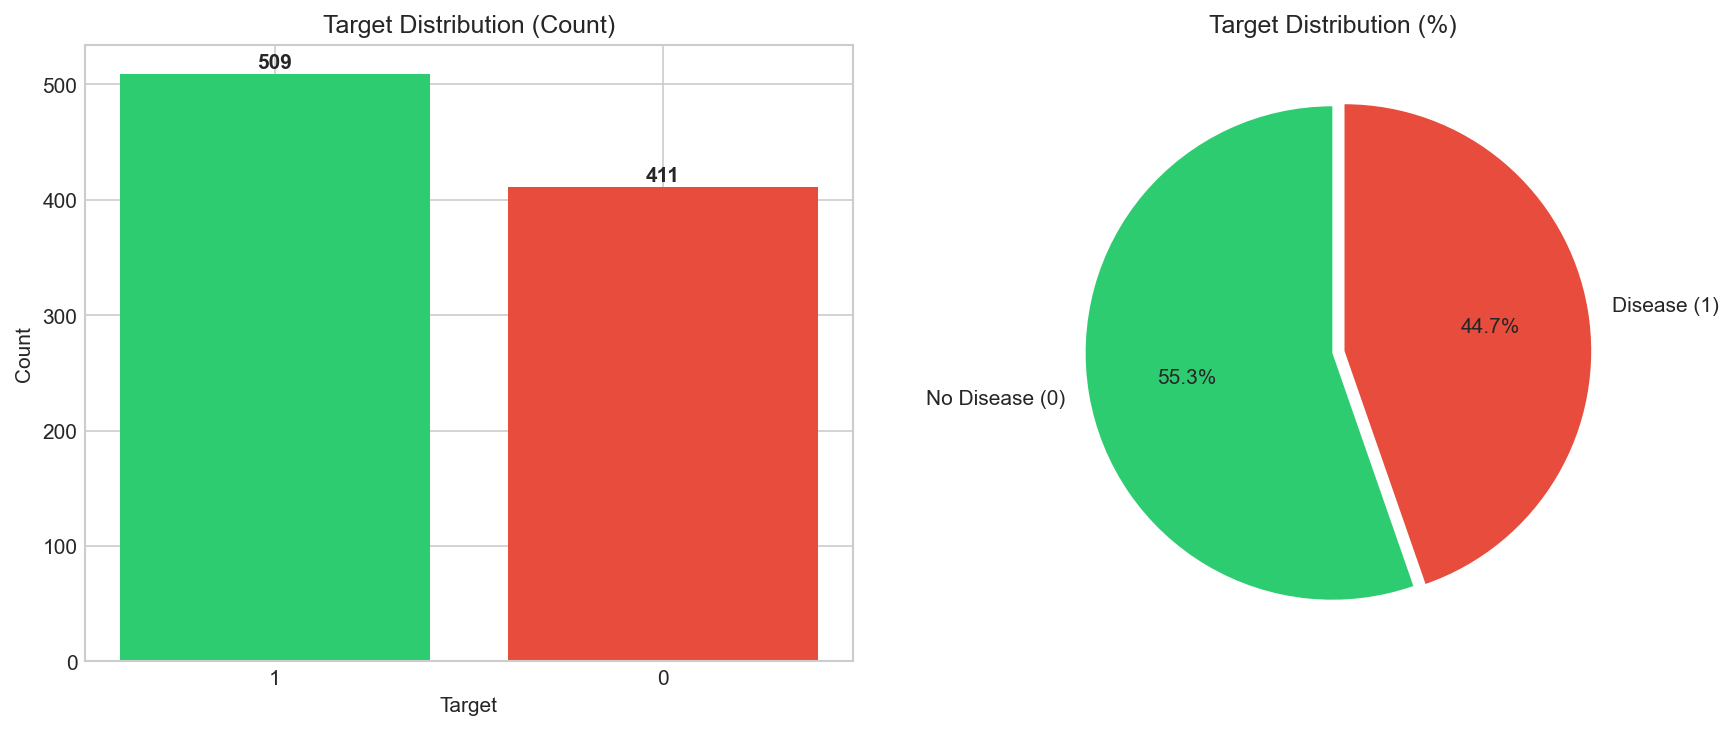
\includegraphics[width=0.7\textwidth]{figs/target_distribution.png}
    \caption{Phân bố biến mục tiêu (Target Distribution): 0 = không bệnh tim, 1 = có bệnh tim.}
    \label{fig:target_dist}
\end{figure}

\subsection{Thống kê mô tả và phân bố dữ liệu}

Hình \ref{fig:numeric_dist} trình bày phân bố histogram của các biến số liên tục trong tập dữ liệu. Qua phân tích, nhóm rút ra một số quan sát đáng chú ý:

\begin{itemize}
    \item \textbf{Tuổi (age):} Phân bố gần dạng chuẩn, tập trung trong khoảng 40--65 tuổi, trung vị khoảng 54 tuổi. Phần đuôi trái (dưới 30 tuổi) rất ít mẫu, cho thấy bệnh tim ít gặp ở nhóm trẻ tuổi, phù hợp với kiến thức y khoa.
    \item \textbf{Huyết áp lúc nghỉ (trestbps):} Phần lớn giá trị nằm trong khoảng 120--140 mmHg (huyết áp bình thường đến tăng huyết áp nhẹ). Có một số giá trị ngoại lai vượt 180 mmHg (tăng huyết áp nặng) và thậm chí giá trị 0 mmHg (rõ ràng là lỗi dữ liệu, cần xử lý).
    \item \textbf{Cholesterol huyết thanh (chol):} Phân bố lệch phải (right-skewed), trung bình khoảng 200--250 mg/dl. Nhiều giá trị ngoại lai phía trên 400 mg/dl, có cả giá trị 0 (có thể do missing hoặc lỗi đo). Cholesterol $\geq$ 240 mg/dl được coi là mức nguy hiểm theo tiêu chuẩn y khoa.
    \item \textbf{Nhịp tim tối đa (thalch):} Phân bố gần chuẩn, trung bình khoảng 137 bpm, dao động từ 60 đến 200 bpm. Bệnh nhân có nhịp tim tối đa thấp (không đạt được nhịp tim mục tiêu khi gắng sức) thường có nguy cơ bệnh tim cao hơn.
    \item \textbf{ST depression (oldpeak):} Phân bố lệch phải rất mạnh, đa số giá trị nằm trong khoảng 0--2 mm. Giá trị $\geq$ 2 mm thường có ý nghĩa bệnh lý và là dấu hiệu quan trọng của thiếu máu cơ tim.
\end{itemize}

\begin{figure}[H]
    \centering
    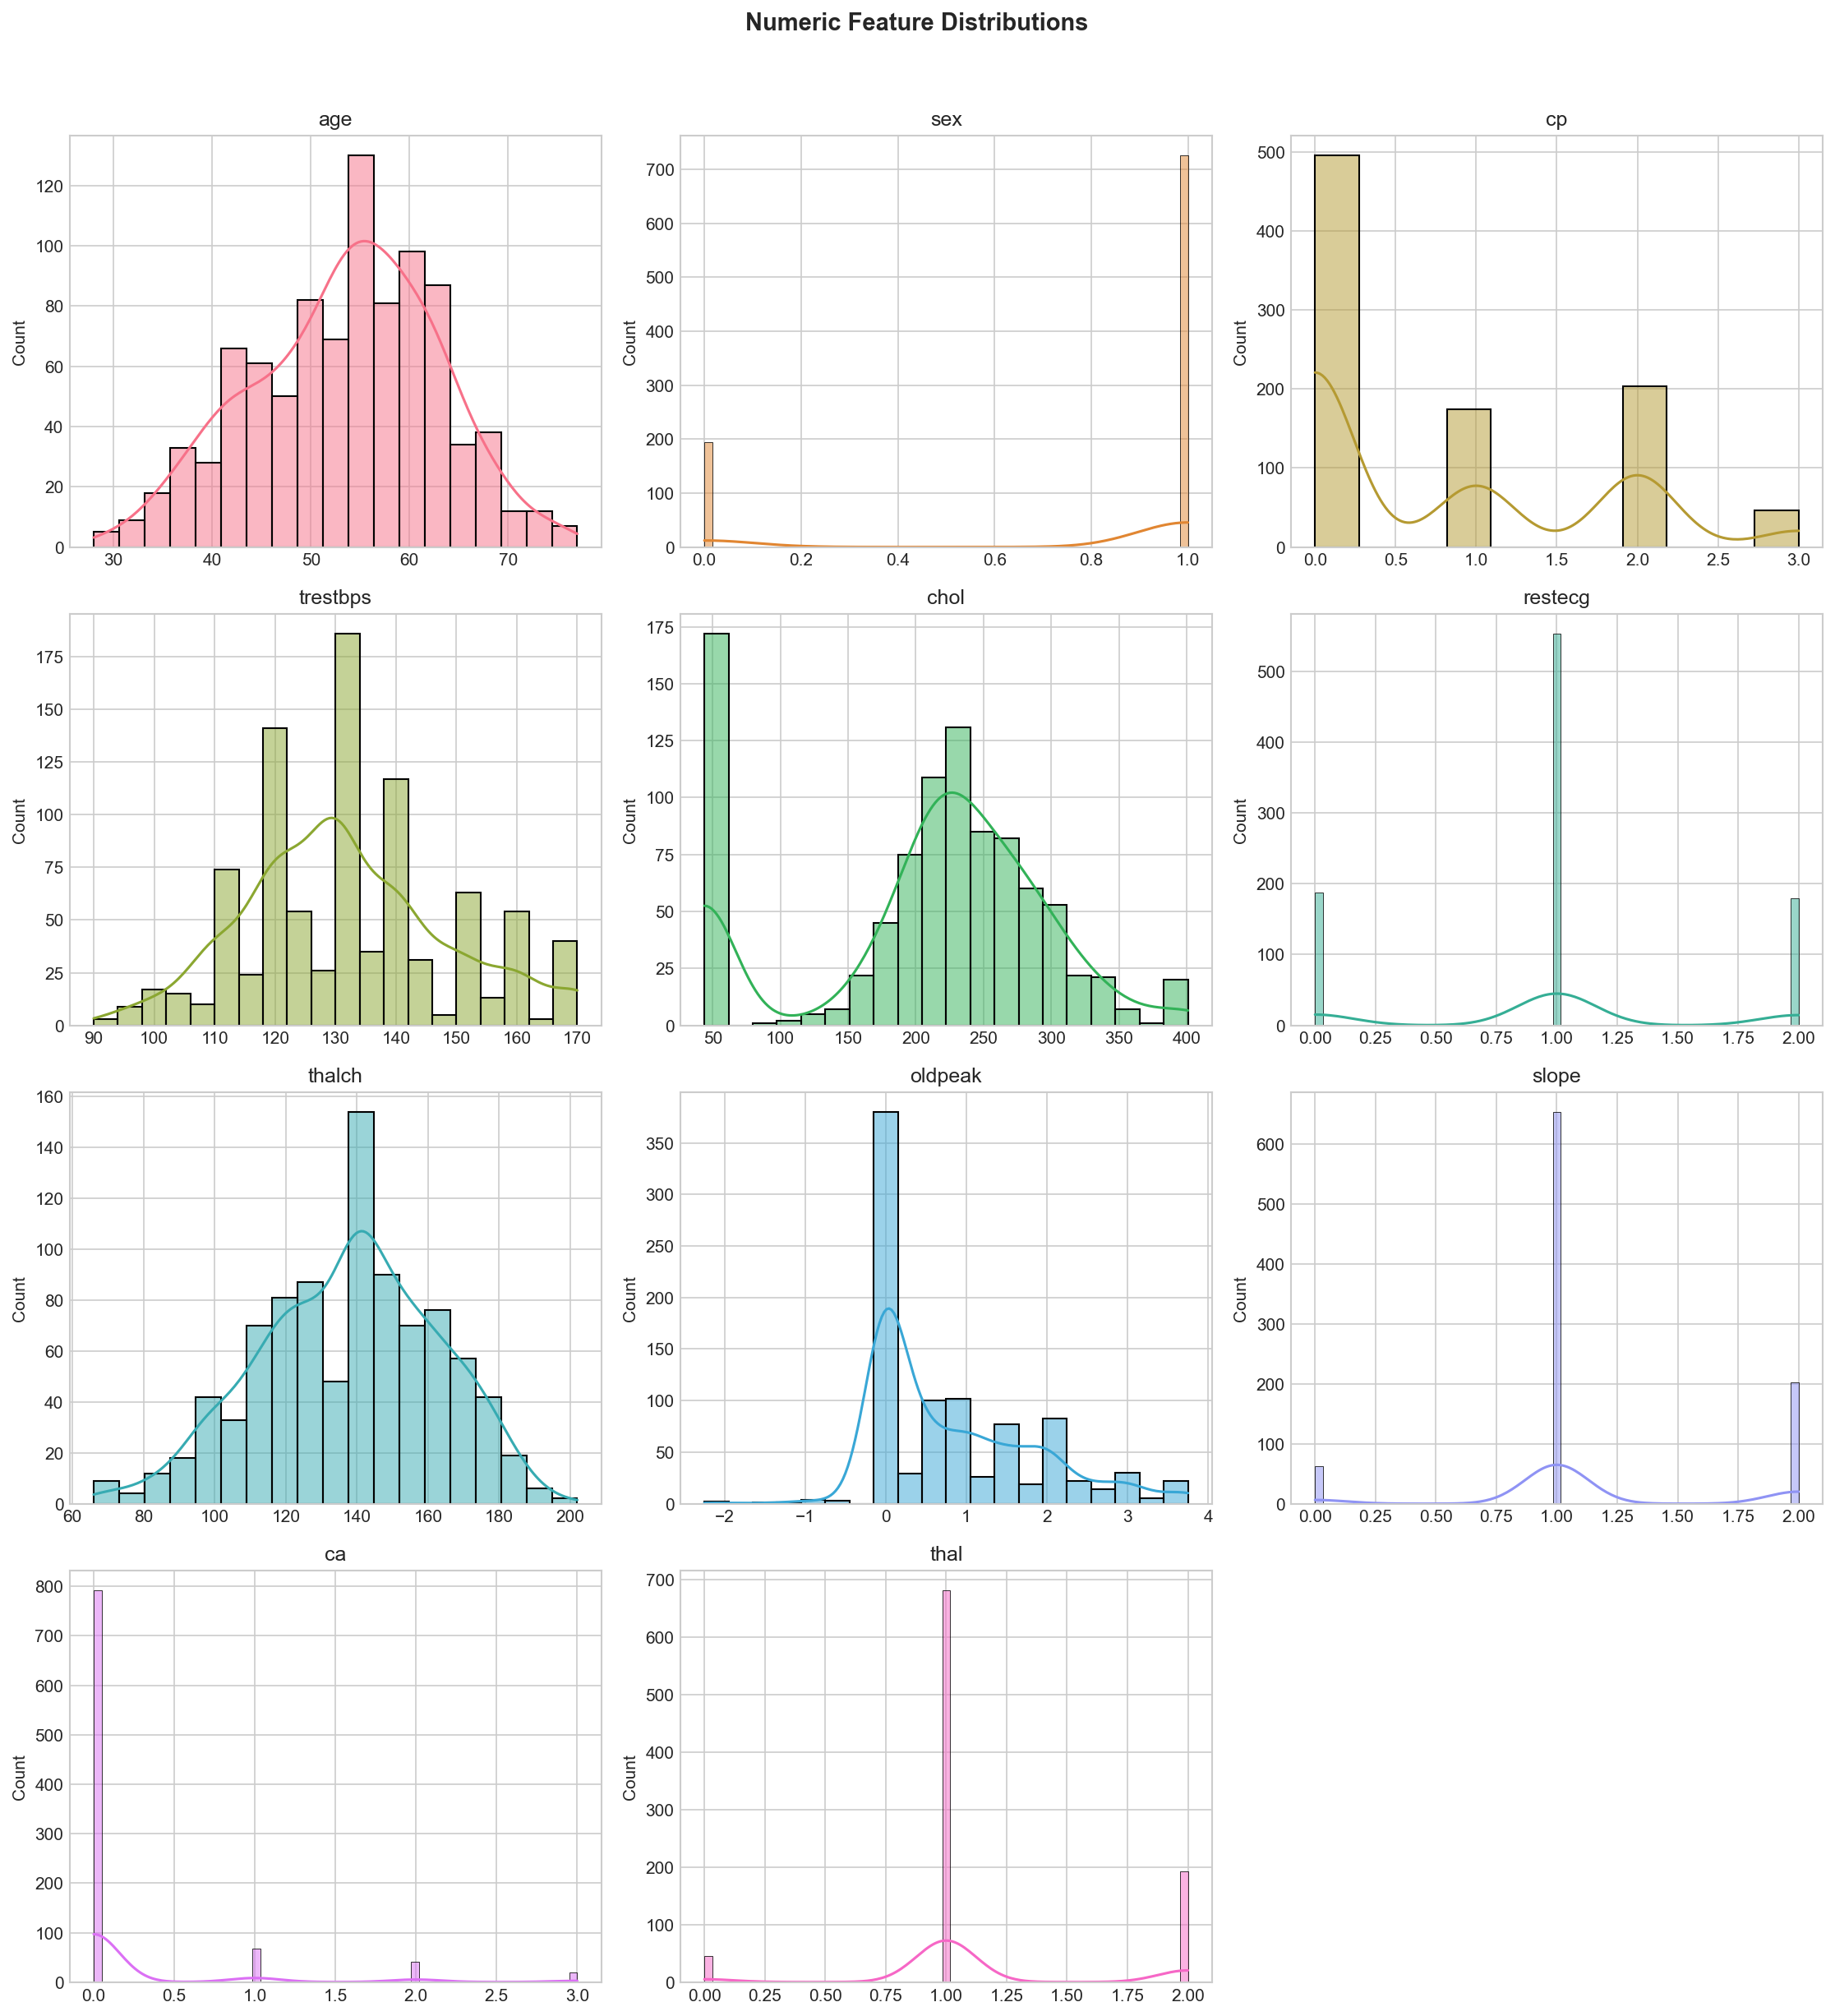
\includegraphics[width=\textwidth]{figs/numeric_distributions.png}
    \caption{Phân bố các biến số liên tục trong tập dữ liệu Heart Disease.}
    \label{fig:numeric_dist}
\end{figure}

\subsection{Tương quan giữa các biến}

Ma trận tương quan Pearson (Hình \ref{fig:corr_matrix}) thể hiện mối quan hệ tuyến tính giữa các biến số. Phân tích cho thấy:

\begin{itemize}
    \item \textbf{Tương quan dương mạnh nhất với target (bệnh tim):} Biến \texttt{oldpeak} (ST depression) và \texttt{ca} (số mạch nhuộm) có tương quan dương với biến mục tiêu, cho thấy bệnh nhân có giá trị cao ở hai biến này thường được chẩn đoán bệnh tim. Đây là hai chỉ số quan trọng trong chẩn đoán lâm sàng bệnh mạch vành.
    \item \textbf{Tương quan âm mạnh nhất với target:} Biến \texttt{thalch} (nhịp tim tối đa) có tương quan âm, nghĩa là bệnh nhân có nhịp tim tối đa thấp (tim không đáp ứng tốt khi gắng sức) thường có nguy cơ bệnh tim cao hơn.
    \item \textbf{Tương quan giữa các đặc trưng:} \texttt{thalch} và \texttt{age} có tương quan âm trung bình (tuổi càng cao thì nhịp tim tối đa khi gắng sức càng giảm -- phù hợp với sinh lý học). \texttt{oldpeak} và \texttt{age} có tương quan dương nhẹ (người lớn tuổi có xu hướng ST depression cao hơn).
    \item \textbf{Multicollinearity:} Không có cặp biến nào có tương quan quá cao ($|r| > 0.8$), cho thấy không cần loại bỏ biến do multicollinearity.
\end{itemize}

\begin{figure}[H]
    \centering
    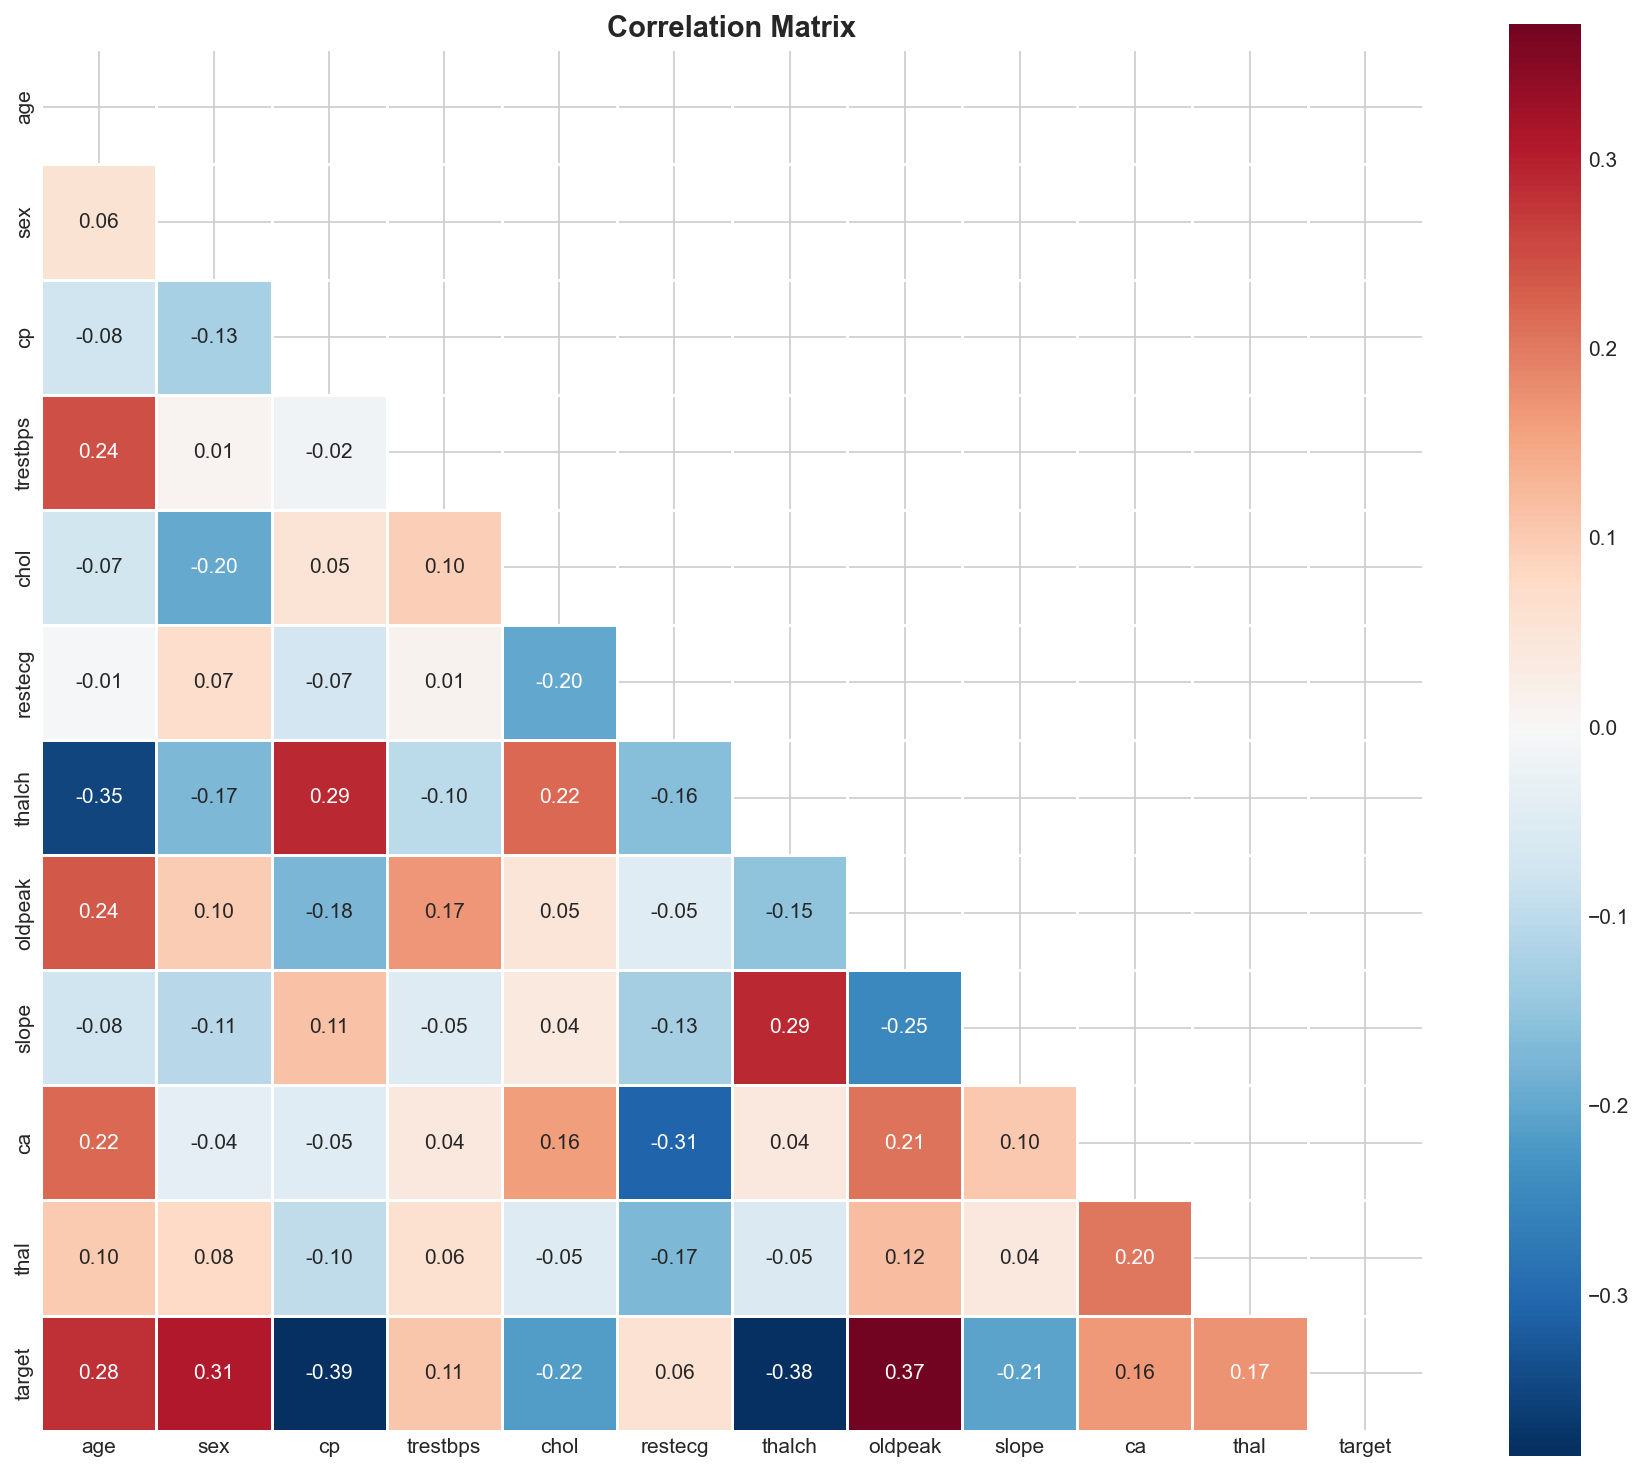
\includegraphics[width=0.85\textwidth]{figs/correlation_matrix.png}
    \caption{Ma trận tương quan Pearson giữa các biến số trong tập dữ liệu.}
    \label{fig:corr_matrix}
\end{figure}

Hình \ref{fig:features_target} minh họa chi tiết hơn mối quan hệ giữa các đặc trưng chính và biến mục tiêu, phân tách theo hai nhóm ``có bệnh'' và ``không bệnh''. Biểu đồ cho thấy sự khác biệt rõ rệt trong phân bố các đặc trưng giữa hai nhóm bệnh nhân, xác nhận rằng các features được chọn có khả năng phân biệt hai lớp.

\begin{figure}[H]
    \centering
    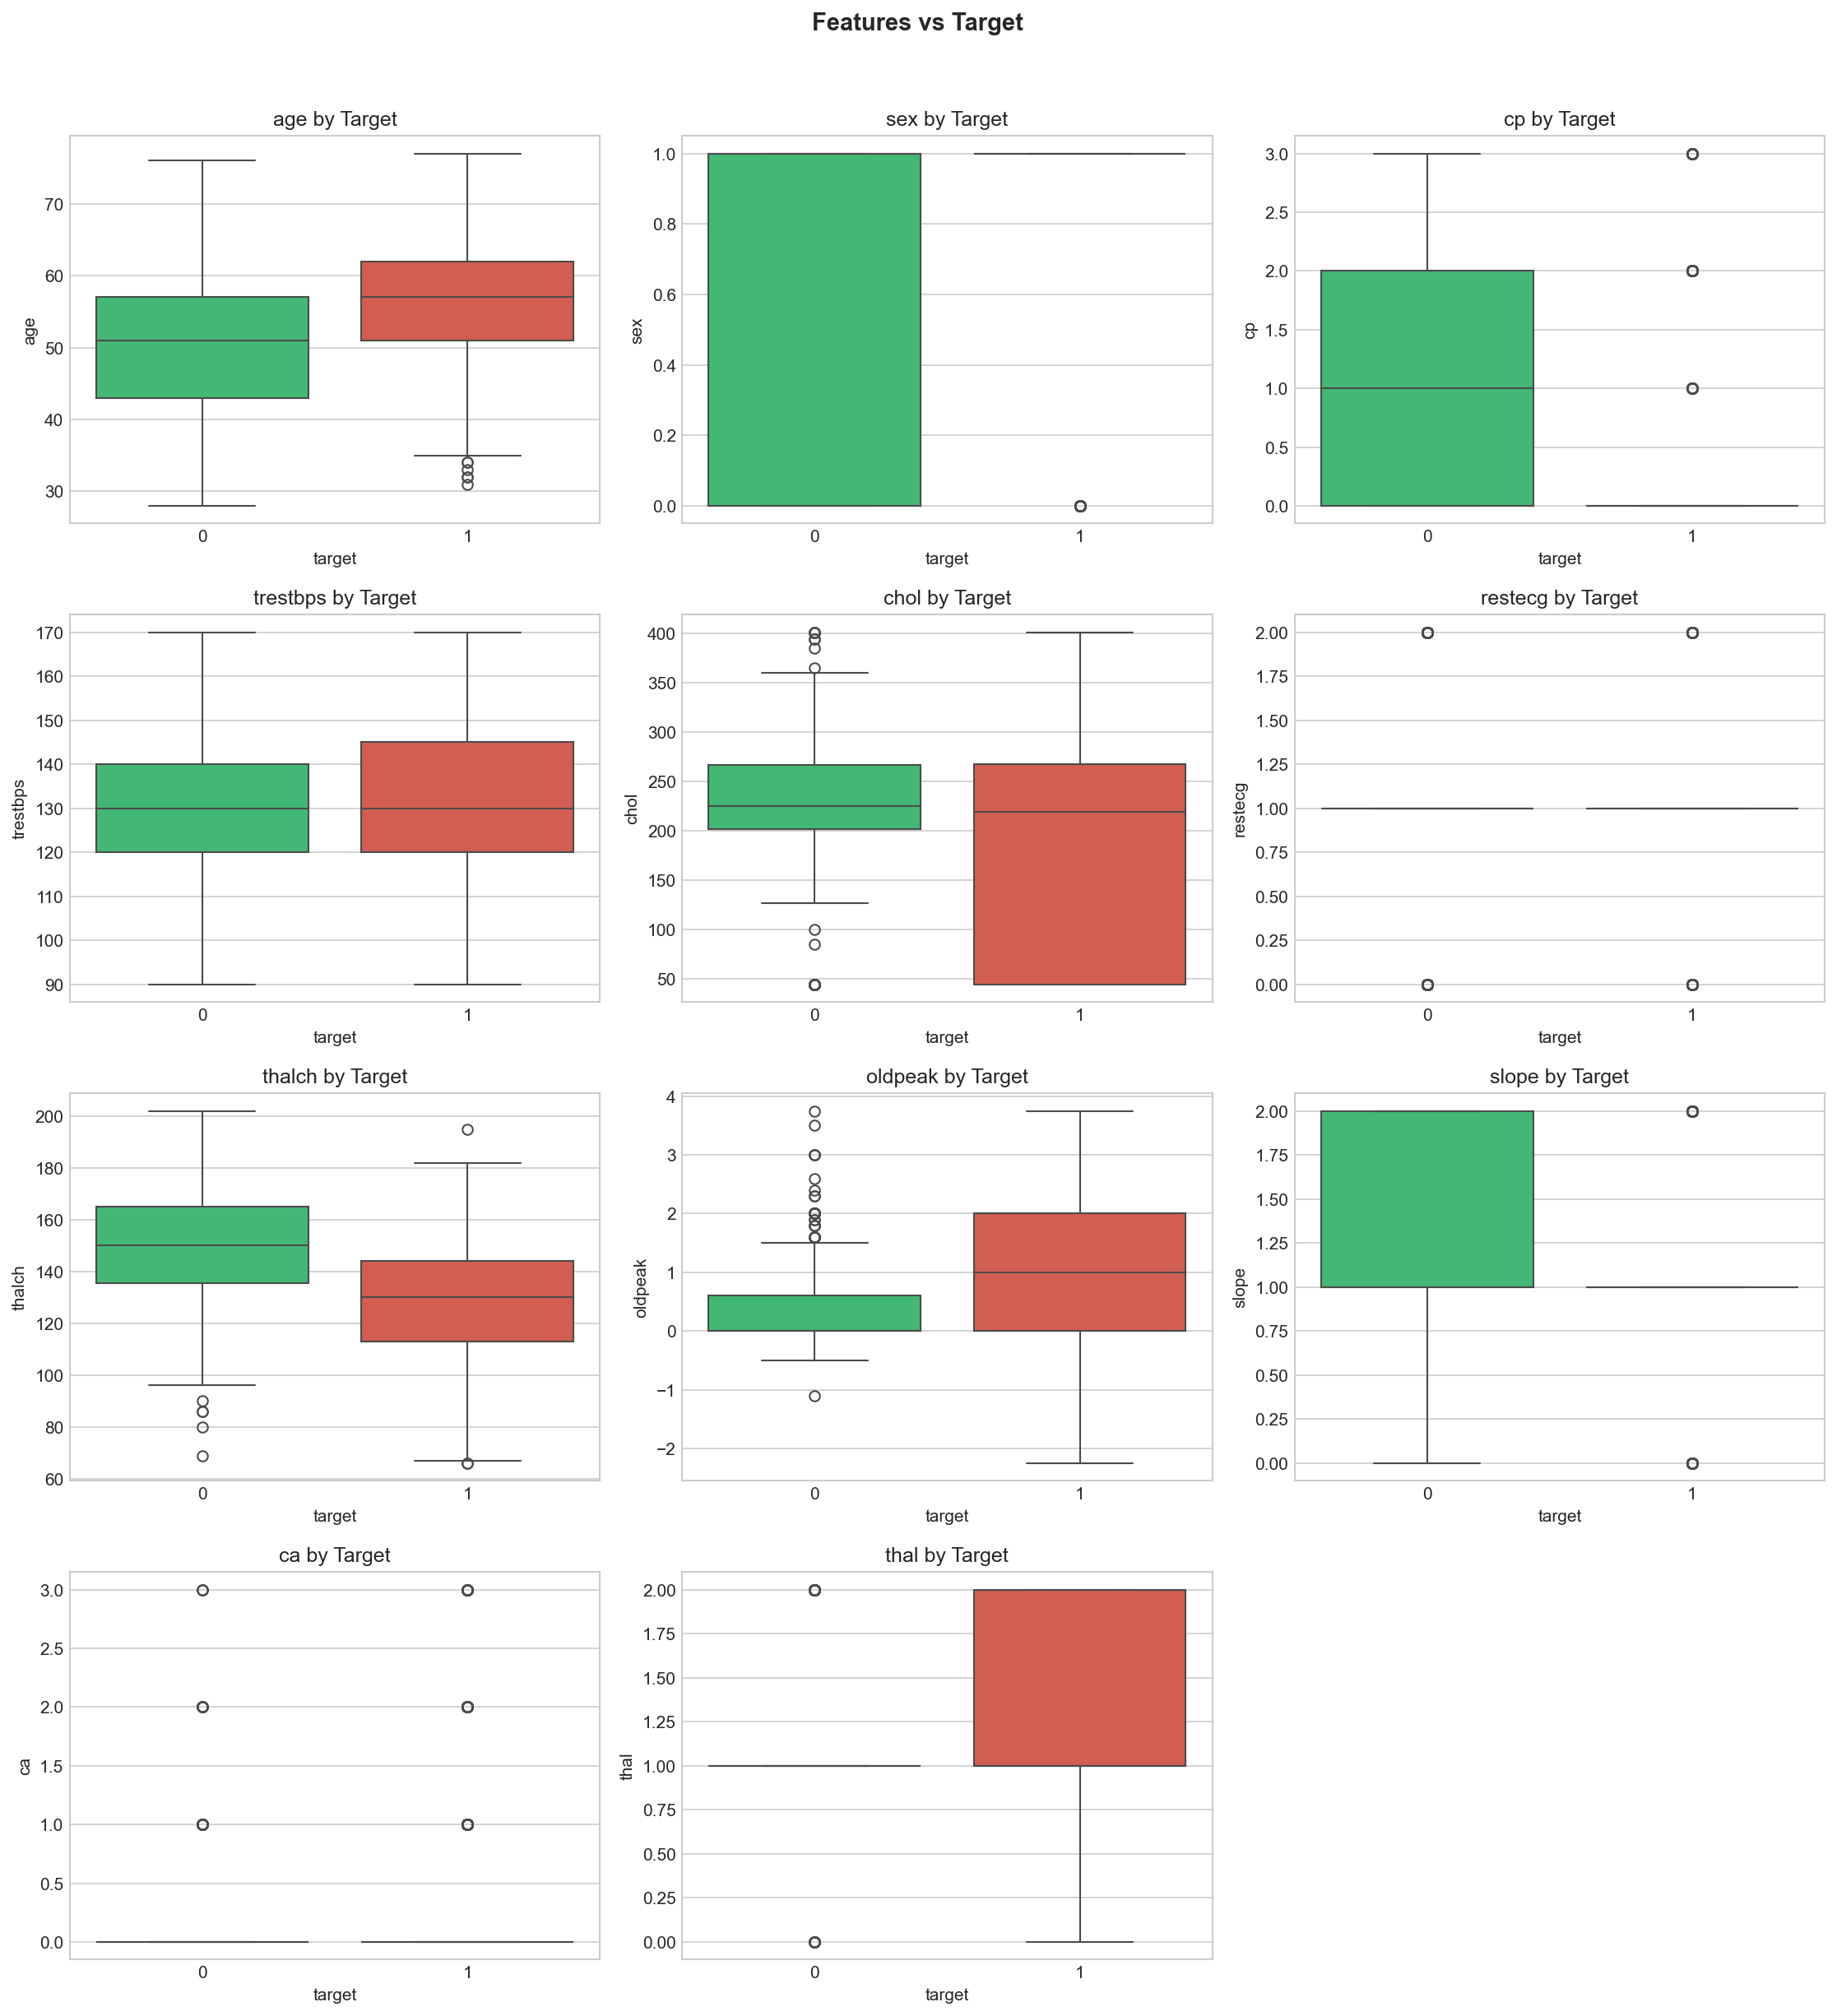
\includegraphics[width=\textwidth]{figs/features_vs_target.png}
    \caption{Phân bố các đặc trưng chính theo biến mục tiêu (0 vs 1).}
    \label{fig:features_target}
\end{figure}

\subsection{Phân tích dữ liệu thiếu (Missing Values)}

Chất lượng dữ liệu là yếu tố then chốt ảnh hưởng đến hiệu quả mô hình. Tập dữ liệu có tổng cộng \textbf{1.759 giá trị thiếu}, phân bố không đều giữa các cột. Hình \ref{fig:missing_values} cho thấy tỷ lệ missing values theo từng cột:

\begin{itemize}
    \item \texttt{ca} (số mạch nhuộm fluoroscopy): $\sim$65\% dữ liệu bị thiếu -- đây là cột có tỷ lệ missing cao nhất. Lý do: xét nghiệm fluoroscopy là phương pháp xâm lấn, tốn kém, không phải bệnh nhân nào cũng được thực hiện.
    \item \texttt{thal} (thalassemia): $\sim$53\% dữ liệu bị thiếu. Tương tự, xét nghiệm thalassemia không phải lúc nào cũng có sẵn ở tất cả các trung tâm y tế.
    \item \texttt{slope} (độ dốc đoạn ST): $\sim$33\% dữ liệu bị thiếu. Chỉ số này cần test gắng sức hoàn chỉnh, một số bệnh nhân không thể hoàn thành test.
    \item \texttt{fbs}, \texttt{restecg}, \texttt{exang}: tỷ lệ missing thấp hơn ($< 15\%$).
    \item \texttt{age}, \texttt{sex}, \texttt{cp}, \texttt{trestbps}: gần như không có missing.
\end{itemize}

\begin{figure}[H]
    \centering
    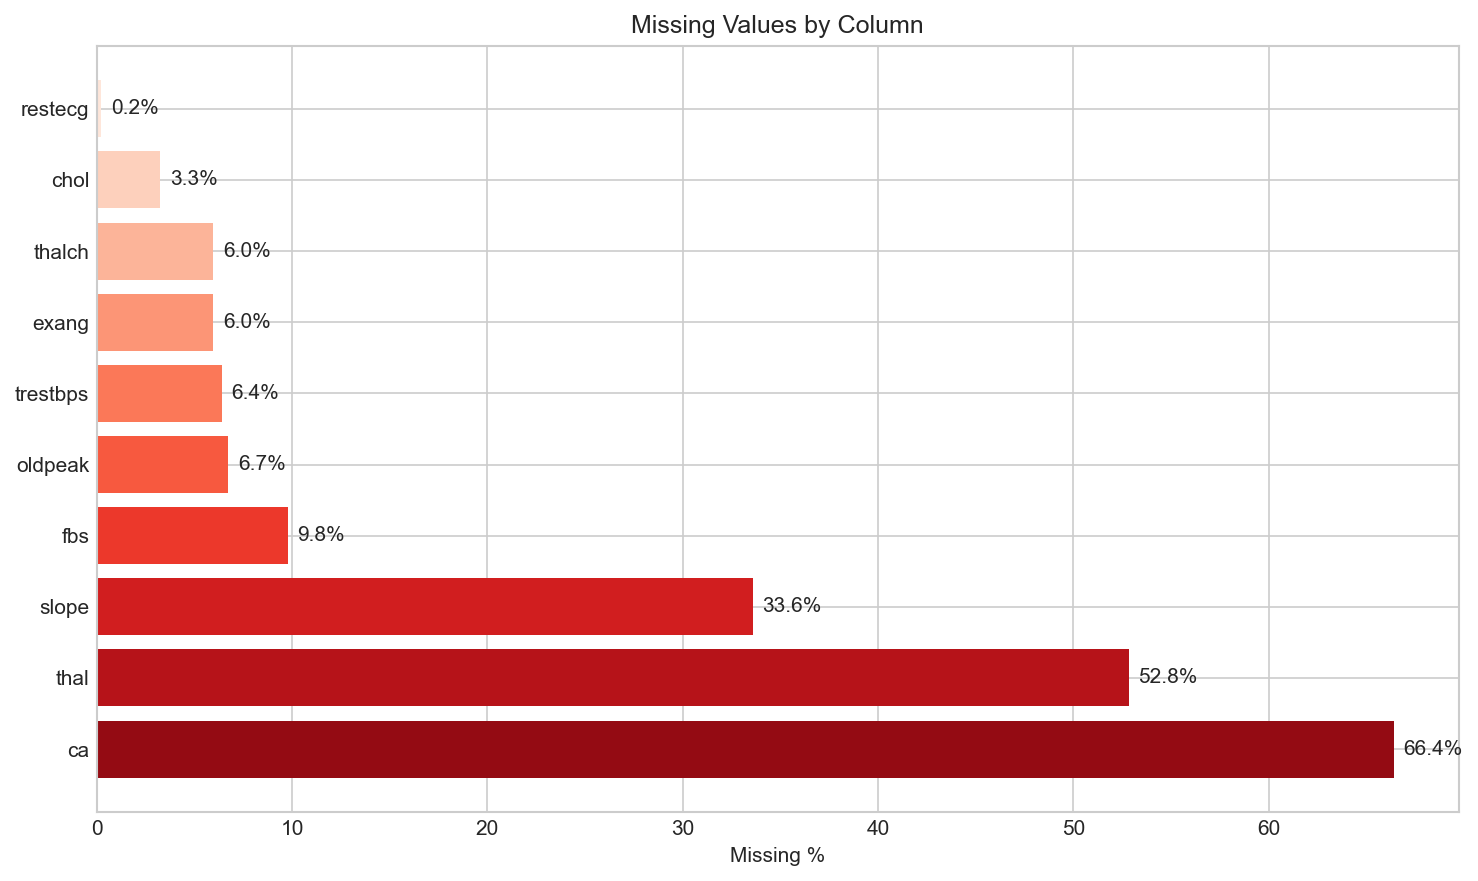
\includegraphics[width=0.8\textwidth]{figs/missing_values.png}
    \caption{Tỷ lệ dữ liệu thiếu (missing values) theo từng cột -- cột \texttt{ca} và \texttt{thal} có tỷ lệ thiếu rất cao.}
    \label{fig:missing_values}
\end{figure}

\subsection{Rủi ro và thách thức của dữ liệu}

Qua toàn bộ quá trình phân tích khám phá, nhóm nhận diện 5 rủi ro và thách thức chính cần xử lý:

\begin{enumerate}
    \item \textbf{Missing values cao ở các biến quan trọng:} Cột \texttt{ca} và \texttt{thal} có tỷ lệ thiếu $>$ 50\%, nhưng đây lại là những đặc trưng y khoa quan trọng, có tương quan mạnh với bệnh tim. Nhóm cần cân nhắc giữa hai chiến lược: loại bỏ cột (mất thông tin) hoặc fill giá trị (thêm noise). Chiến lược fill median/mode được chọn để giữ tối đa thông tin.
    
    \item \textbf{Mất cân bằng lớp nhẹ:} Tỷ lệ 55:45 giữa hai lớp không quá nghiêm trọng, nhưng cần xử lý để tránh mô hình thiên vị. Nhóm sử dụng hai kỹ thuật bổ sung: SMOTE (tạo mẫu tổng hợp cho lớp thiểu số) và \texttt{class\_weight=balanced} (điều chỉnh trọng số lớp trong thuật toán).
    
    \item \textbf{Data leakage tiềm ẩn:} Một sai lầm phổ biến trong Data Science là áp dụng preprocessing (scaling, SMOTE) trên toàn bộ dataset trước khi chia train/test. Điều này dẫn đến data leakage -- thông tin từ tập test ``rò rỉ'' vào tập train, làm kết quả đánh giá trở nên lạc quan hơn thực tế. Nhóm đảm bảo: StandardScaler được fit trên train, transform trên test; SMOTE chỉ áp dụng trên train.
    
    \item \textbf{Dữ liệu đa nguồn:} Dữ liệu từ 4 trung tâm y tế ở 3 quốc gia khác nhau, mỗi nơi có quy trình thu thập, thiết bị đo lường và population demographics khác nhau. Điều này tạo ra selection bias và measurement bias tiềm ẩn. Cột \texttt{dataset} được loại bỏ trong modeling, nhưng bias vẫn có thể tồn tại ở mức ngầm.
    
    \item \textbf{Giá trị ngoại lai (Outliers):} Các biến cholesterol, huyết áp có giá trị ngoại lai đáng kể (bao gồm cả giá trị 0 -- có khả năng là lỗi dữ liệu). Nhóm sử dụng phương pháp IQR (Interquartile Range) để phát hiện và clip outliers, giữ nguyên kích thước mẫu thay vì loại bỏ hàng.
\end{enumerate}
